\tikzset{every picture/.style={line width=0.75pt}} %set default line width to 0.75pt        

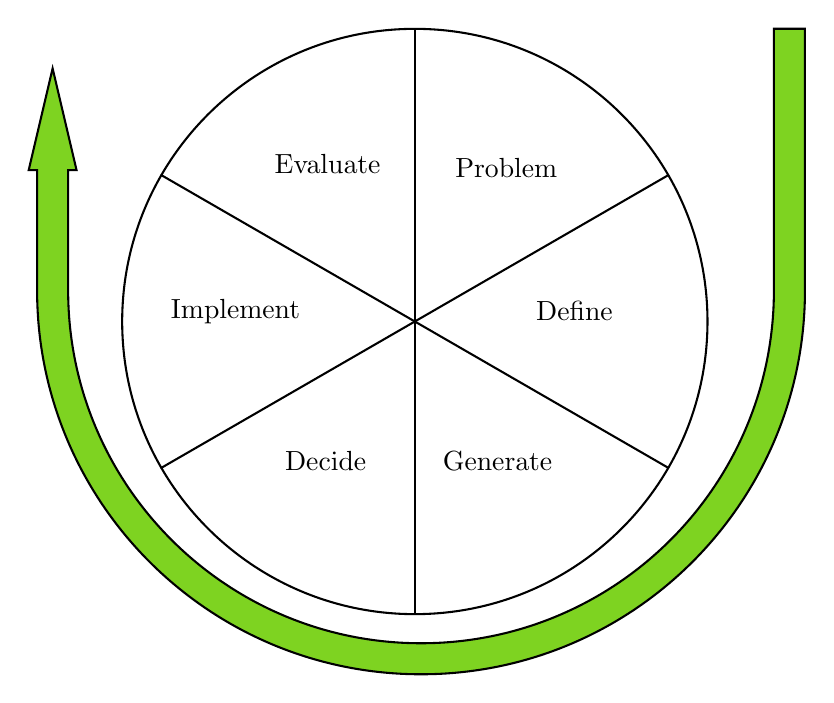
\begin{tikzpicture}[x=0.75pt,y=0.75pt,yscale=-1,xscale=1]
%uncomment if require: \path (0,429); %set diagram left start at 0, and has height of 429

%Shape: Circle [id:dp22618983135620052] 
\draw   (183,215) .. controls (183,137.13) and (246.13,74) .. (324,74) .. controls (401.87,74) and (465,137.13) .. (465,215) .. controls (465,292.87) and (401.87,356) .. (324,356) .. controls (246.13,356) and (183,292.87) .. (183,215) -- cycle ;
%Straight Lines [id:da21765413351304574] 
\draw    (324,215) -- (324,74) ;
%Straight Lines [id:da11891026729648879] 
\draw    (324,215) -- (324,356) ;
%Shape: Boxed Line [id:dp49474400628170856] 
\draw    (324,215) -- (446.47,285.71) ;
%Shape: Boxed Line [id:dp5884296541863099] 
\draw    (446.47,144.29) -- (324,215) ;
%Shape: Boxed Line [id:dp04693235846756805] 
\draw    (201.53,144.29) -- (324,215) ;
%Shape: Boxed Line [id:dp40804207399259274] 
\draw    (324,215) -- (201.53,285.71) ;
%U Turn Arrow [id:dp7489586044285481] 
\draw  [fill={rgb, 255:red, 126; green, 211; blue, 33 }  ,fill opacity=1 ] (511.96,73.94) -- (511.96,200) .. controls (511.96,302.16) and (429.14,384.97) .. (326.99,384.97) -- (326.99,384.97) .. controls (224.83,384.97) and (142.01,302.16) .. (142.01,200) -- (142.01,142.04) -- (137.97,142.04) -- (149.49,93.06) -- (161.01,142.04) -- (156.97,142.04) -- (156.97,200) .. controls (156.97,293.9) and (233.09,370.02) .. (326.99,370.02) -- (326.99,370.02) .. controls (420.88,370.02) and (497,293.9) .. (497,200) -- (497,73.94) -- cycle ;

% Text Node
\draw (342,135) node [anchor=north west][inner sep=0.75pt]   [align=left] {Problem};
% Text Node
\draw (381,204) node [anchor=north west][inner sep=0.75pt]   [align=left] {Define};
% Text Node
\draw (336,276) node [anchor=north west][inner sep=0.75pt]   [align=left] {Generate};
% Text Node
\draw (260,276) node [anchor=north west][inner sep=0.75pt]   [align=left] {Decide};
% Text Node
\draw (205,203) node [anchor=north west][inner sep=0.75pt]   [align=left] {Implement};
% Text Node
\draw (255,133) node [anchor=north west][inner sep=0.75pt]   [align=left] {Evaluate};


\end{tikzpicture}
